人地关系是人类活动与地球表层系统的相互影响与反馈作用\cite{wu1991,li2016d},但人水关系却不能被简单定义为“人类活动与水圈的相互影响与反馈作用”。
地球表层系统作为开放复杂巨系统,四大圈层之内或之间有着复杂的能量交换和物质流动,人类无法脱离其它任何圈层,人类活动对其它圈层的影响也会随着地球表层过程而深远影响水圈。
如从这个角度出发,人地关系与人水关系将完全等价,且都指向人类与地球表层系统所共同构成的人-地复合系统。
但在人地关系研究中,无论是人类与地球表层要素间的单向影响还是反馈循环,研究者约定俗成会将着眼点放在某个“影响/反馈作用实体”上,给出$Y = f(X_1, X_2, \dots)$的显式表达,而绝无可能穷尽此复合系统的全部作用关系。
因此出于研究需要,本章为“人水关系”给出如下广义定义:
% TODO 定义
水圈要素过程作为自变量或因变量时,人类活动与地球表层系统的相互影响与反馈作用。
根据此定义,若人类活动不直接改变水圈要素过程、且其间接导致的水圈变化也不会被人类活动所考虑时,便不再是人水关系的范畴。

根据上述广义定义,水也是塑造人类世界观及行为模式的重要元素,相关理论或经验研究(如社会科学中“水的社会性”研究)也属于广义的人水关系,绝不是从某一时刻才产生的事物,因此本研究题目强调其“演变过程”。
水圈或水文系统被人类活动改造则是人水关系的一种表现,相关理论或经验研究(如流域“自然-社会”二元水循环理论\cite{wang2006, wang2016})所强调的多是近现代人类活动影响水圈要素过程后的一种人水关系表现形式。
因本研究侧重“流域可持续性”层面,不再考虑人类对自然水过程影响微乎其微的史前时期,仅将时间尺度聚焦在人类有能力改造水圈要素过程,因而存在“自然-社会”二元水循环的时期。

% 开题报告
\begin{figure}[!htb]
    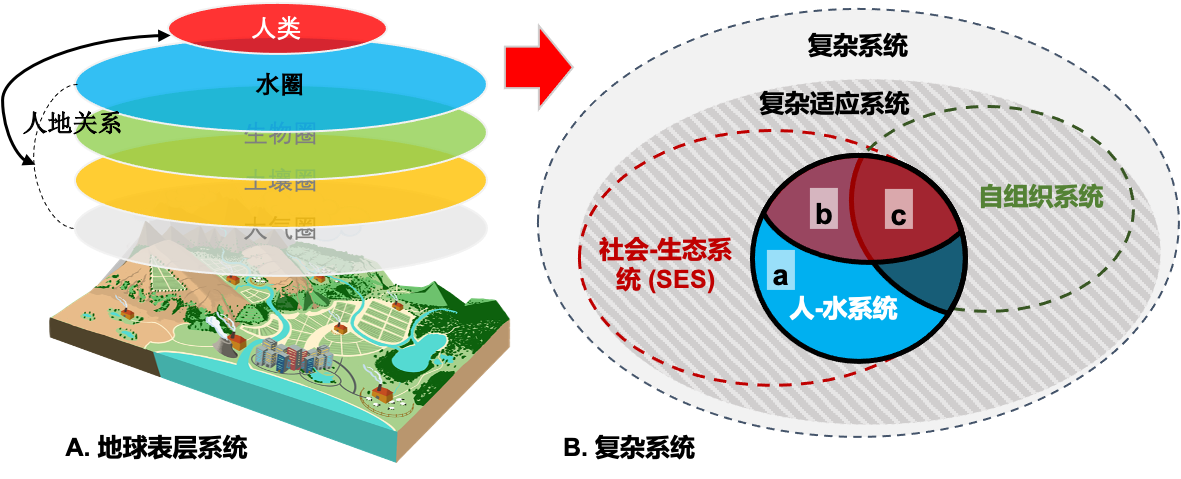
\includegraphics[width=\textwidth]{img/ch2/ch2_definitions.png}
    \caption[主要研究内容与相关概念]{主要研究内容与相关概念。本研究主要关注的人-水系统(Human-water system)与概念范围更广的社会-生态系统(Social-ecological system, SES)都是典型的复杂系统(Complex system),因此基于复杂系统的建模也常常以人-水系统为研究对象。(a)本研究首先以黄河为研究案例,梳理人-水系统演变过程;(b)在其基础上重点分析水的资源属性下发生变化的人-水关系。(c)最后在SES分析框架下,利用基于复杂系统建模的技术手段,对资源属性引导下的人-水关系演变过程进行机制模拟。}\label{ch2:fig:definitions}
\end{figure}
